% Fig. 3: panel a (circuit, drawn here) and panels b, c (fig3bc.pdf from matplotlib, included at 100%).
% Width 7.05 in = 17.907 cm, height 2.05 in = 5.207 cm. Panel a is 2.65 in = 6.731 cm wide.
% Titles sit 0.367 cm below the top edge, as in the matplotlib panels.
\documentclass[border=0pt]{standalone}
% Shared TikZ style for the schematics. Same typeface, size (8 pt) and palette as figstyle.py:
% blue = memory / reservoir dynamics, red = noise and the limit, purple = input, greys = neutral.
\usepackage[T1]{fontenc}
\usepackage{helvet}
\renewcommand{\familydefault}{\sfdefault}
\usepackage{amsmath,amssymb,bm}
\usepackage{tikz}
\usetikzlibrary{arrows.meta,calc,decorations.pathreplacing,patterns.meta,shapes.geometric,shadows}
\definecolor{cInk}{HTML}{1A1A1A}
\definecolor{cBlue}{HTML}{3C7FE0}
\definecolor{cBlueDark}{HTML}{1D4C9C}
\definecolor{cBlueLight}{HTML}{8DB8F0}
\definecolor{cBlueFill}{HTML}{DDE9F9}
\definecolor{cRed}{HTML}{EF4B3B}
\definecolor{cRedDark}{HTML}{B8301F}
\definecolor{cRedFill}{HTML}{FCE3DE}
\definecolor{cPurple}{HTML}{9B4FE0}
\definecolor{cPurpleDark}{HTML}{6B2CAB}
\definecolor{cPurpleFill}{HTML}{EFE2FB}
\definecolor{cGreyDark}{HTML}{4A4A4A}
\definecolor{cGrey}{HTML}{8C8C8C}
\definecolor{cGreyLight}{HTML}{B4B4B4}
\definecolor{cGreyFill}{HTML}{EDEDED}
\definecolor{cShadow}{HTML}{B5B5B5}
\tikzset{
  every node/.style={font=\fontsize{8}{9.6}\selectfont},
  lbl/.style={font=\fontsize{8}{9.6}\selectfont},
  ttl/.style={font=\fontsize{8}{9.6}\selectfont,anchor=base west,inner sep=0pt},
  ttlr/.style={font=\fontsize{8}{9.6}\selectfont,anchor=base east,inner sep=0pt},
  wire/.style={line width=0.65pt,cInk},
  ublk/.style={draw=cInk,line width=0.6pt,fill=cBlue,rounded corners=1.6pt},
  iblk/.style={draw=cInk,line width=0.6pt,rounded corners=1.6pt,preaction={fill=cPurple},
    pattern={Lines[angle=55,distance=2.2pt,line width=0.85pt]},pattern color=white},
  nbox/.style={draw=cInk,line width=0.55pt,fill=cRed,rounded corners=1.1pt},
  feat/.style={draw=cInk,line width=0.6pt,fill=white,rounded corners=2pt,inner sep=1.6pt,
    minimum width=0.98cm,minimum height=0.44cm},
  legbox/.style={draw=cInk,line width=0.8pt,fill=white,rounded corners=2.4pt,
    drop shadow={shadow xshift=1.2pt,shadow yshift=-1.2pt,fill=cShadow,opacity=1}},
  arr/.style={line width=0.65pt,-{Stealth[length=3.6pt,width=3.2pt]}},
  brc/.style={decorate,decoration={brace,amplitude=2.6pt},line width=0.55pt},
}
\newcommand{\Discard}[3][cInk]{%
  \draw[line width=0.75pt,#1] (#2,{#3-0.1}) -- (#2,{#3+0.1});
  \draw[line width=0.75pt,#1] ({#2+0.05},{#3-0.064}) -- ({#2+0.05},{#3+0.064});
  \draw[line width=0.75pt,#1] ({#2+0.1},{#3-0.03}) -- ({#2+0.1},{#3+0.03});}
\providecommand{\ket}[1]{|#1\rangle}
\providecommand{\nrm}[2]{\lvert #1\rvert_{#2}}

\begin{document}
\begin{tikzpicture}[x=1cm,y=1cm]
\useasboundingbox (0,0) rectangle (17.907,5.207);
\node[anchor=north west,inner sep=0pt,outer sep=0pt] at (6.731,5.207) {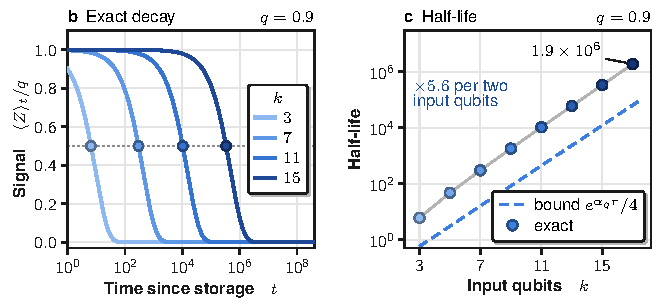
\includegraphics{fig3bc.pdf}};
\node[ttl] at (0,4.840) {\textbf{a}\enspace Repetition-code reservoir};
\begin{scope}[shift={(0.16,0)}]
\def\yc{3.86}\def\yb{3.54}\def\ya{3.16}\def\yaa{2.84}\def\yab{2.52}\def\yx{1.98}\def\yxa{1.66}\def\yxb{1.34}
\def\xw{2.40}\def\xn{4.18}\def\xd{4.55}
% reservoir unitary U = write + swap (blue background), input register (purple background)
\fill[cBlueFill,rounded corners=2.5pt] (2.10,1.10) rectangle (3.84,4.08);
\node[text=cBlueDark,anchor=south] at (2.97,4.10) {$U$};
\fill[cPurpleFill,rounded corners=2.5pt] (1.28,2.36) rectangle (1.94,4.08);
\node[text=cPurpleDark,anchor=south] at (1.61,4.10) {input register};
\node[anchor=east] at (1.92,\yc) {$\ket{c}$};
\node[anchor=east] at (1.92,\yb) {$\ket{b}$};
\foreach \y in {\ya,\yaa,\yab} \node[anchor=east] at (1.92,\y) {$\ket{0}$};
\foreach \y in {\yc,\yb,\ya,\yaa,\yab} \draw[wire] (1.94,\y) -- (\xd,\y);
\foreach \y in {\yx,\yxa,\yxb} \draw[wire] (1.28,\y) -- (4.80,\y);
\foreach \y in {\yx,\yxa,\yxb} \draw[wire,-{Stealth[length=2.8pt,width=2.6pt]}] (4.70,\y) -- (4.92,\y);
% write gate: F of the memory content (or the bit b) into the ancillas
\draw[line width=0.7pt,cBlueDark] (\xw,\yxb) -- (\xw,\yc);
\foreach \y in {\yx,\yxa,\yxb,\yc,\yb} \fill[cBlueDark] (\xw,\y) circle (1.6pt);
\foreach \y in {\ya,\yaa,\yab} {\draw[cBlueDark,line width=0.7pt,fill=white] (\xw,\y) circle (0.09);
  \draw[cBlueDark,line width=0.7pt] ({\xw-0.09},\y) -- ({\xw+0.09},\y) (\xw,{\y-0.09}) -- (\xw,{\y+0.09});}
\node[draw=cBlueDark,line width=0.6pt,fill=white,rounded corners=1.2pt,inner sep=1.4pt] at (\xw,2.25) {$F$};
% swaps of ancillas and memory qubits
\foreach \sx/\sa/\sm in {2.98/3.16/1.98,3.26/2.84/1.66,3.54/2.52/1.34}{
  \draw[line width=0.7pt,cBlueDark] (\sx,\sa) -- (\sx,\sm);
  \foreach \y in {\sa,\sm} \draw[line width=0.95pt,cBlueDark] ({\sx-0.065},{\y-0.065}) -- ({\sx+0.065},{\y+0.065})
    ({\sx-0.065},{\y+0.065}) -- ({\sx+0.065},{\y-0.065});}
% noise on every qubit
\foreach \y in {\yc,\yb,\ya,\yaa,\yab,\yx,\yxa,\yxb} \path[nbox] ({\xn-0.095},{\y-0.095}) rectangle ({\xn+0.095},{\y+0.095});
% discard of the input register at the next input injection
\foreach \y in {\yc,\yb,\ya,\yaa,\yab} {\Discard{\xd}{\y}}
\draw[brc] (4.80,{\yc+0.12}) -- (4.80,{\yab-0.12})
  node[midway,right=2.4pt,align=left,text=cPurpleDark]{discarded:\\old copies\\leave};
\draw[brc] (5.04,{\yx+0.12}) -- (5.04,{\yxb-0.12})
  node[midway,right=2.4pt,align=left]{refreshed\\copies};
\draw[brc] (1.22,{\yxb-0.12}) -- (1.22,{\yx+0.12})
  node[midway,left=2.4pt,align=right]{memory,\\$r$ qubits};
% column labels
\node[text=cBlueDark,anchor=base] at (\xw,0.80) {write};
\node[text=cBlueDark,anchor=base] at (3.26,0.80) {swap};
\node[text=cRedDark,anchor=base] at (\xn,0.80) {noise};
\end{scope}
\node[align=left,anchor=south west,inner sep=0pt] at (0.0,0.02) {$F=\mathrm{maj}(x)$ for a blank input ($c=0$),\\$F=b$ to store the bit $b$ ($c=1$)};
\end{tikzpicture}
\end{document}
